\documentclass{article}
\usepackage[margin=1in]{geometry}
\usepackage{amsmath,amsthm,amssymb}
\usepackage{bbm,enumerate,mathtools}
\usepackage{tikz,pgfplots}
\usepackage{chessboard}
\usepackage[hidelinks]{hyperref}
\usepackage{multicol} % Problem 35
\usepackage{xstring} % Difficulty command
\usetikzlibrary{shapes.geometric}

\newenvironment{question}{\begin{trivlist}\item[\textbf{Question.}]}{\end{trivlist}}
\newenvironment{note}{\begin{trivlist}\item[\textbf{Note.}]}{\end{trivlist}}
\newenvironment{references}{\begin{trivlist}\item[\textbf{References.}]}{\end{trivlist}}
\newenvironment{related}{\begin{trivlist}\item[\textbf{Related.}]\end{trivlist}\begin{enumerate}}{\end{enumerate}}

\newcommand\score[1]{
\pgfmathsetmacro\pgfxa{#1+1}
\tikzstyle{scorestars}=[
  star,
  star points=5,
  star point ratio=2.25,
  draw,
  inner sep=3pt,
  anchor=outer point 5
]
  \begin{tikzpicture}[baseline]
    \draw[opacity=0] (0,-0.5) rectangle (0,0.2); % Workaround for whitespace at the bottom.
    \foreach \i in {1,...,4} {
      \pgfmathparse{(\i<=#1?"yellow":"gray")}
      \edef\starcolor{\pgfmathresult}
      \draw (\i*4.5ex,0) node[name=star\i,scorestars,fill=\starcolor]  {};
    }
  \end{tikzpicture}
}

\newcommand{\difficulty}[1]{%
  \IfEqCase{#1}{%
      {1}{
        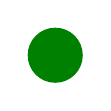
\begin{tikzpicture}[scale=0.7, baseline=0.9mm]%
          \definecolor{slopegreen}{rgb}{0.0, 0.5, 0.0}%
          \fill[slopegreen] (0.5,0.5) circle (0.5);%
        \end{tikzpicture}%
      }%
      {2}{
        
\begin{tikzpicture}[scale=0.7, baseline=0.9mm]%
          \definecolor{slopeblue}{rgb}{0.0, 0.44, 1.00}
          \fill[slopeblue] (0,0) rectangle (1,1);%
        \end{tikzpicture}%
      }%
      {3}{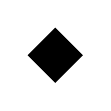
\begin{tikzpicture}[scale=0.7, baseline=0.9mm]\fill (0,0.5)--(0.5, 0)--(1,0.5)--(0.5,1)--cycle; \end{tikzpicture}}%
      {4}{
\begin{tikzpicture}[scale=0.7, baseline=0.9mm]\fill (0.25,0)--(0,0.5)--(0.25,1)--(0.5,0.5)--cycle; \fill (0.75,0)--(0.5,0.5)--(0.75,1)--(1,0.5)--cycle;\end{tikzpicture}}%
      % you can add more cases here as desired
  }[\PackageError{difficulty}{Undefined difficulty level: #1}{}]%
}%
\newcommand{\rating}[2]{\difficulty{#1}\\\score{#2}\\}


\begin{document}
\rating{2}{4}

Richard Stanley guesses that determining whether or not an arbitrary polyomino can be used to tile a rectangle is undecidable---that is, there is not a general purpose algorithm that can do so. We call such polyominoes ``rectifiable.''

Here we define something different: we say that a polyomino is ``toroidal'' if it can be used to tile a rectangular torus grid. All rectifiable polyominoes are toroidal, and all polyominoes that tile the plane with two dimensions of translational symmetry are toroidal.

\begin{figure}[ht!]
  % \includegraphics[width=0.3\linewidth]{assets/138_problem/embedded_torus.png}
  \begin{tikzpicture}
    \node at (0,0) {\includegraphics[width=0.3\linewidth]{assets/138_problem/unfolded.png}};
    \node at (5.5,0) {\includegraphics[width=0.257\linewidth]{assets/138_problem/flat_torus.png}};
    \draw[thick] (7.6,-1.4) rectangle (3.4,1.4);
    \draw[red,line width=3, ->] (3.4,-1.4) -- (5.5,-1.4);
    \draw[red,line width=3, ->] (3.4,-1.4) -- (6,-1.4);
    \draw[red,line width=3] (3.4,-1.4) -- (7.6,-1.4);
    \draw[red,line width=3, ->] (3.4,1.4) -- (5.5,1.4);
    \draw[red,line width=3, ->] (3.4,1.4) -- (6,1.4);
    \draw[red,line width=3] (3.4,1.4) -- (7.6,1.4);

    \draw[blue,line width=3, ->] (3.4,-1.4) -- (3.4,0.2);
    \draw[blue,line width=3] (3.4,-1.4) -- (3.4,1.4);
    \draw[blue,line width=3, ->] (7.6,-1.4) -- (7.6,0.2);
    \draw[blue,line width=3] (7.6,-1.4) -- (7.6,1.4);

    \node at (11,0) {\includegraphics[width=0.3\linewidth]{assets/138_problem/embedded_torus.png}};
\end{tikzpicture}
  \caption{
    An illustration of a toroidable $6$-omino that is not rectifiable.
  }
\end{figure}

\begin{question}
  For each $n$, what is the toroidable $n$-omino with the largest minimal torus?
\end{question}

\begin{related}
  \item What about polyiamonds? Polyhexes? Other polyforms?
  \item Suppose we want to $k$-color the torus so that no color is adjacent to itself by an edge (alternatively, vertex). What is the largest minimal coloring over all $n$-ominoes.
\end{related}

\begin{references}
  \item MathOverflow.
\end{references}
\end{document}
